\documentclass[aspectratio=169, 12pt]{beamer}

\usepackage{lmodern}
\usepackage{hyperref}
\usepackage{graphicx}
\usepackage{booktabs}
\usepackage[authordate,maxcitenames=1,backend=biber,doi=false,isbn=false,url=false]{biblatex-chicago}
\renewcommand*{\nameyeardelim}{\addcomma\addspace}
% \addbibresource{discrimination.bib}

\usepackage{amsmath}
\usepackage{amssymb}
\usepackage{amsthm}
\usepackage{bm}
\usepackage{bbm}
\usepackage{mathtools}
\setbeamertemplate{theorems}[numbered]
\newtheorem{proposition}{Proposition}
\newtheorem{assumption}{Assumption}

\DeclareMathOperator*{\plim}{plim}
\DeclareMathOperator*{\var}{var}
\DeclareMathOperator*{\cov}{cov}

\newcommand{\indep}{\perp \!\!\! \perp}
\newcommand{\R}{\mathbb{R}}
\newcommand{\I}{\mathbbm{1}}
\newcommand{\argmax}{\mathop{\rm arg~max}\limits}
\newcommand{\argmin}{\mathop{\rm arg~min}\limits}

% preambles for tables
\usepackage{booktabs}
\usepackage{adjustbox}
\usepackage{caption}
\captionsetup{labelformat=empty}
\usepackage{tikz}
\usetikzlibrary{calc}
\newcommand{\tikzmark}[1]{\tikz[overlay,remember picture] \node (#1) {};}
\newcommand{\DrawBox}[1][]{%
    \tikz[overlay,remember picture]{
    \draw[#1,thick]
      ($(left)+(-0.2em,0.9em)$) rectangle
      ($(right)+(0.2em,-0.3em)$);}
}
\usepackage[group-separator={,}]{siunitx}
\usepackage{longtable}
\usepackage{rotating}
\usepackage{threeparttable}

\newcommand{\backupbegin}{
   \newcounter{framenumberappendix}
   \setcounter{framenumberappendix}{\value{framenumber}}
}
\newcommand{\backupend}{
   \addtocounter{framenumberappendix}{-\value{framenumber}}
   \addtocounter{framenumber}{\value{framenumberappendix}} 
}

\usepackage{silence}
\WarningFilter{latexfont}{Font shape}
\WarningFilter{biblatex}{Patching footnotes failed}

\usetheme{Boadilla}
\usecolortheme{orchid}
\usefonttheme{professionalfonts}

\setbeamertemplate{section in toc}[sections numbered]
\setbeamertemplate{itemize item}[default]
\setbeamertemplate{itemize subitem}[square]
\setbeamertemplate{enumerate items}[default]
\setbeamertemplate{navigation symbols}{}
\setbeamertemplate{itemize/enumerate body begin}{\normalsize}
\setbeamertemplate{itemize/enumerate subbody begin}{\normalsize}
\setbeamertemplate{itemize/enumerate subsubbody begin}{\normalsize}
\setbeamerfont{title}{size=\large}
\setbeamerfont{institute}{size=\small}
\setbeamercovered{dynamic}


\title[Survival analysis]{Topics on survival analysis}
\author[Konan Hara]{Konan Hara}
\institute[Arizona]{University of Arizona}
\date{\today}
\begin{document}

	\begin{frame}[plain]
	\titlepage
	\end{frame}

	\begin{frame}
	\frametitle{Outline}
	\tableofcontents
	\end{frame}

	\AtBeginSection[]
	{
	   \begin{frame}
	       \frametitle{Outline}
	       \tableofcontents[currentsection]
	   \end{frame}
	}

	\section{Introduction}

	\begin{frame}
	\frametitle{Introduction\footnote{The following contents are primarily based on Wang, Li, and Reddy (2019, ACM Computing Surveys).}}
	\begin{itemize}
	\item The goal of survival analysis is to analyze and model data where the outcome is the time until an event of interest occurs, $T$.
	\item $T$ can always be transformed into an occurrence of the event within a specified period.
	\item The advantages and disadvantages of using either survival analysis methods or other rudimentary regression methods should be weighed.

	\end{itemize}
	\end{frame}

	\begin{frame}
	\frametitle{Pros and Cons}
	\begin{itemize}
	\item Survival analysis can deal with
	\begin{itemize}
	\item Censoring
	\item Time-dependent covariates
	\item Competing risks

	\end{itemize}
	\item However, the costs are that
	\begin{itemize}
	\item Assumptions for causal inference are strong
	\item Models are complicated and not so intuitive
	\item Machine learning methods are difficult to apply

	\end{itemize}
	\end{itemize}
	
	\end{frame}

	\begin{frame}
	\frametitle{Topics}
	\centering{
	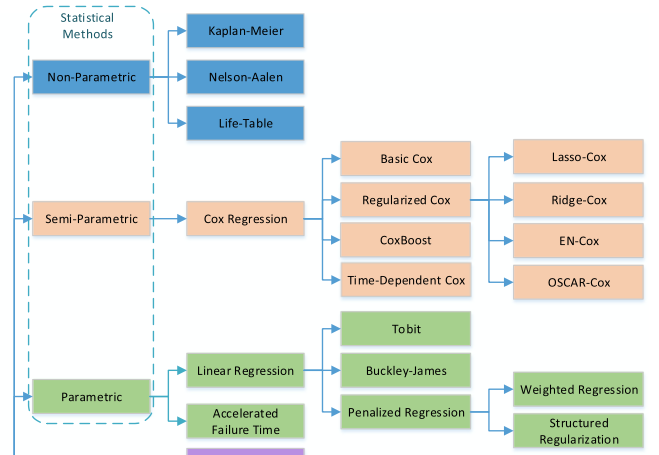
\includegraphics[width=11cm]{fig/Wang_et_al_Fig3_1.png}
	}
	\end{frame}

	\begin{frame}
	\frametitle{Topics}
	\centering{
	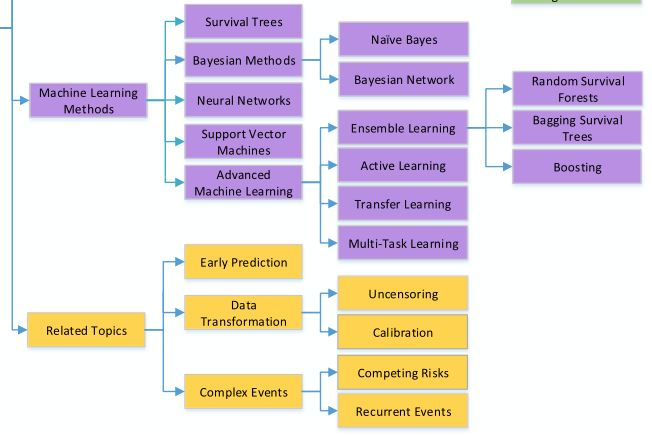
\includegraphics[width=11cm]{fig/Wang_et_al_Fig3_2.png}
	}
	\end{frame}

	\section{Definition}

	\begin{frame}
	\frametitle{Survival Data and Censoring}
	\centering{
	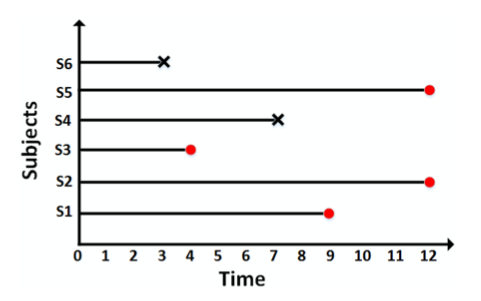
\includegraphics[width=9cm]{fig/Wang_et_al_Fig1.png}\\
	X marks: event occurrence\\
	Red dots: censored
	}
	\end{frame}

	\begin{frame}
	\frametitle{Problem Statement}
	\begin{itemize}
	\item Data: a triplet $(X_i, y_i, \delta_i)$
	\begin{itemize}
	\item $i \in \{1 \dots N\}$: individual 
	\item $X_i \in \mathbb{R}^p$: independent variables
	\item $\delta_i$: $0$ if censored and $1$ if otherwise 
	\item $y_i$: $T_i$ if $\delta_i = 1$ and $C_i$ if otherwise 
	\item $T_i$: survival time
	\item $C_i$: censored time

	\end{itemize}
	\item Goal: estimate the effect of some elements of $X$ on $T$ or predict $T$ with $X$

	\end{itemize}
	\end{frame}

	\begin{frame}
	\frametitle{Survival and Hazard Function}
	\begin{itemize}
	\item Survival function: $S(t) = \Pr(T \geq t)$
	\item Cumulative distribution function: $F(t) = 1 - S(t)$
	\item Density function:
	\begin{eqnarray*}
	f(t) = \frac{d}{dt}F(t) = \lim_{\Delta t \to 0}\frac{\Pr(t \leq T < t + \Delta t)}{\Delta t}
	\end{eqnarray*}
	\item Hazard function:
	\begin{eqnarray*}
	h(t) = \lim_{\Delta t \to 0}\frac{\Pr(t \leq T < t + \Delta t | T \geq t)}{\Delta t} = \frac{f(t)}{S(t)}
	\end{eqnarray*}

	\end{itemize}
	\end{frame}

	\begin{frame}
	\frametitle{Survival and Hazard Function}
	\centering{
	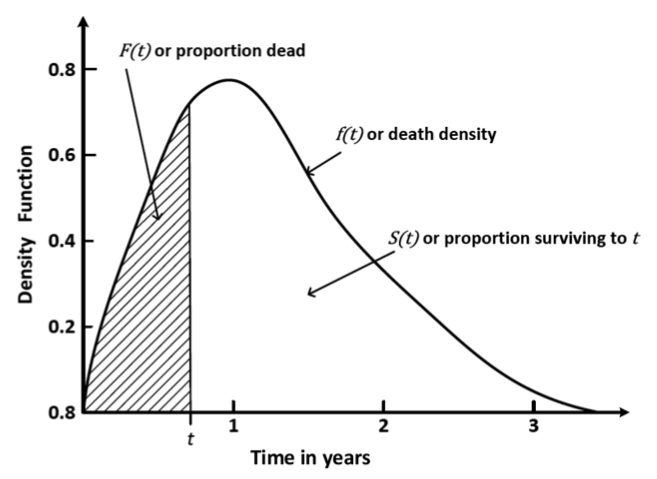
\includegraphics[width=10.5cm]{fig/Wang_et_al_Fig2.png}
	}
	\end{frame}

	\begin{frame}
	\frametitle{Identification}
	\begin{itemize}
	\item Consider a simple nonparametric estimator of $f(t)$:
	\begin{eqnarray*}
	\hat{f}(t) &=& \frac{1}{N} \sum_{i=1}^N I(t \leq T_i < t + \Delta t)\\
	&\to& \lim_{\Delta t \to 0}\frac{\Pr(t \leq T < t + \Delta t, \delta = 1)}{\Delta t}
	\end{eqnarray*}
	\item Unfortunately,
	\begin{eqnarray*}
	\Pr(t \leq T < t + \Delta t, \delta = 1) < \Pr(t \leq T < t + \Delta t)
	\end{eqnarray*}
	unless $\delta_i = 1$ for all $i$, no censoring.

	\end{itemize}
	\end{frame}

	\begin{frame}
	\frametitle{Identification}
	\begin{itemize}
	\item Thus, we cannot get a consistent estimator for $f(t)$.
	\item How about $h(t)$?
	\item $R(t)$: set of individuals considered to be ``at risk'' at time $t$
	\item $r(t)$: number of individuals considered to be ``at risk'' at time $t$, $|R(t)|$

	\end{itemize}
	\end{frame}

	\begin{frame}
	\frametitle{Identification}
	Then, a simple nonparametric estimator of $h(t)$ is
	\begin{eqnarray*}
	&\phantom{=}& \hat{h}(t)\\
	&=& \frac{1}{r(t)} \sum_{i \in R(t)} I(t \leq T_i < t + \Delta t)\\
	&\to& \lim_{\Delta t \to 0}\frac{\Pr(t \leq T < t + \Delta t, \delta = 1 | T \geq t, \delta = 1)}{\Delta t}
	\end{eqnarray*}
	What is the condition to be
	\begin{eqnarray*}
	&\phantom{=}& \Pr(t \leq T < t + \Delta t, \delta = 1 | T \geq t, \delta = 1)\\
	&=& \Pr(t \leq T < t + \Delta t | T \geq t)?
	\end{eqnarray*}

	\end{frame}

	\begin{frame}
	\frametitle{Identification}
	If $T \indep \delta$, then
	\begin{eqnarray*}
	&\phantom{=}& \Pr(t \leq T < t + \Delta t, \delta = 1 | T \geq t, \delta = 1)\\
	&=& \frac{\Pr(t \leq T < t + \Delta t, \delta = 1)}{\Pr(T \geq t, \delta = 1)}\\
	&=& \frac{\Pr(t \leq T < t + \Delta t) \Pr(\delta = 1)}{\Pr(T \geq t) \Pr(\delta = 1)}\\
	&=& \Pr(t \leq T < t + \Delta t | T \geq t).
	\end{eqnarray*}
	Thus, we can get a consistent estimator for $h(t)$.

	\end{frame}

	\begin{frame}
	\frametitle{From $h(t)$ to $f(t)$}
	As
	\begin{eqnarray*}
	&\phantom{\Leftrightarrow}& h(t) = \frac{f(t)}{1-F(t)} = -\frac{d\log \{1-F(t)\}}{dt}\\
	&\Leftrightarrow& F(t) = 1-\exp \left\{-\int_0^t h(\tau) d\tau \right\}\\
	&\Leftrightarrow& f(t) = h(t) \exp \left\{-\int_0^t h(\tau) d\tau \right\},
	\end{eqnarray*}
	we can calculate $f(t)$ from $h(t)$.

	\end{frame}


	\section{Statistical Methods}

	\begin{frame}
	\frametitle{Nonparametric Models: Kaplan-Meier Curve}
	Let event times be $T_1 < T_2 < \dots < T_K$ for $N$ individuals and consider a specific event time $T_j$:
	\begin{itemize}
	\item $d(T_j)$: observed events
	\item $c(T_j)$: censored individuals between $T_{j}$ and $T_{j+1}$
	\item then, $r(T_j) = r(T_{j-1}) - d(T_{j-1}) - c(T_{j-1})$

	\end{itemize}

	\end{frame}

	\begin{frame}
	\frametitle{Kaplan-Meier Curve}
	\begin{itemize}
	\item Conditional probability of surviving beyond $T_j$:
	\begin{eqnarray*}
	p(T_j) = \frac{r(T_j) - d(T_j)}{r(T_j)}
	\end{eqnarray*}
	\item The estimator of $S(t) = \Pr(T \geq t)$ is given as
	\begin{eqnarray*}
	\hat{S}(t) = \prod_{j: T_j < t} p(T_j)
	\end{eqnarray*}
	\item Nonparametric: no functional form specification

	\end{itemize}

	\end{frame}

	\begin{frame}
	\frametitle{Kaplan-Meier Curve---Covariates}
	\begin{itemize}
	\item The effect of $X$ can be quantified by stratification.
	\item Time-dependent covariates $X(t)$ can be incorporated as well.
	\item Set of individuals considered to be ``at risk'' at time $t$ will be $R(t, X(t))$.

	\end{itemize}

	\end{frame}

	\begin{frame}
	\frametitle{Kaplan-Meier Curve}
	\centering{
	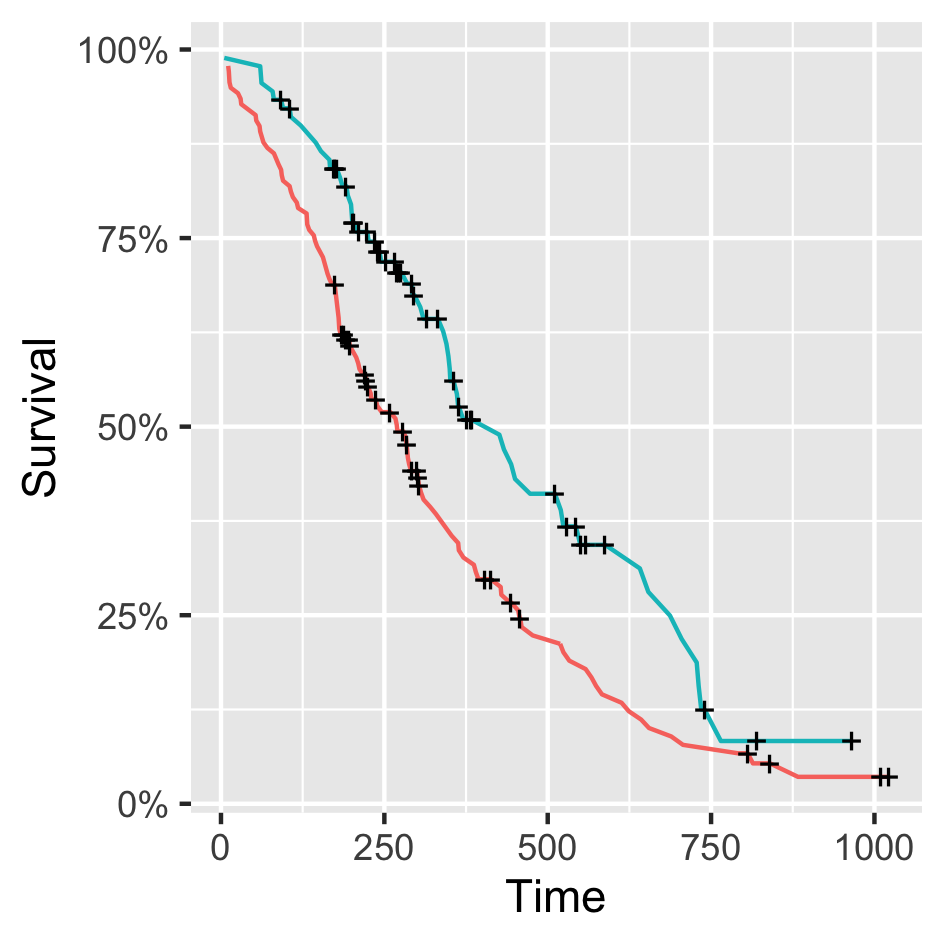
\includegraphics[width=7.5cm]{fig/km.png}
	}
	\end{frame}

	\begin{frame}
	\frametitle{Semiparametric Models: Cox Model}
	\begin{itemize}
	\item Semiparametric models can give more efficient estimates than nonparametric models
	\item Hazard function $h(t,X_i)$ follows the proportional hazards assumption:
	\begin{eqnarray*}
	h(t,X_i) = h_0(t) \exp(X_i \beta)
	\end{eqnarray*}
	\item Proportional hazards:
	\begin{eqnarray*}
	\frac{h(t,X_i)}{h(t,X_j)} = \frac{h_0(t) \exp(X_i \beta)}{h_0(t) \exp(X_j \beta)} = \frac{\exp(X_i \beta)}{\exp(X_j \beta)}
	\end{eqnarray*}

	\end{itemize}

	\end{frame}

	\begin{frame}
	\frametitle{Cox Model}
	\begin{itemize}
	\item Semiparametric: baseline hazard function $h_0(t)$ can be left unspecified in the estimation of $\beta$
	\item $h_0(t)$ can be estimated nonparametrically
	\item Likelihood of event time $T_i$:
	\begin{eqnarray*}
	\frac{h(T_i,X_i) \Delta t}{\sum_{j \in R(T_i)} h(T_i,X_j) \Delta t}
	\end{eqnarray*}
	\item Maximum partial likelihood estimator:
	\begin{eqnarray*}
	\hat{\beta} = \argmax_{\beta} \prod_{i=1}^N \left\{\frac{\exp(X_i \beta)}{\sum_{j \in R_i} \exp(X_j \beta)} \right\}^{\delta_i}
	\end{eqnarray*}

	\end{itemize}

	\end{frame}

	\begin{frame}
	\frametitle{Time-Dependent Cox Model}
	\begin{itemize}
	\item Cox model can handle time-dependent covariates
	\item Hazard function:
	\begin{eqnarray*}
	h(t,X_i(t)) = h_0(t) \exp(X_i(t) \beta)
	\end{eqnarray*}

	\end{itemize}

	\end{frame}

	\begin{frame}
	\frametitle{Time-Dependent Cox Model}
	\centering{
	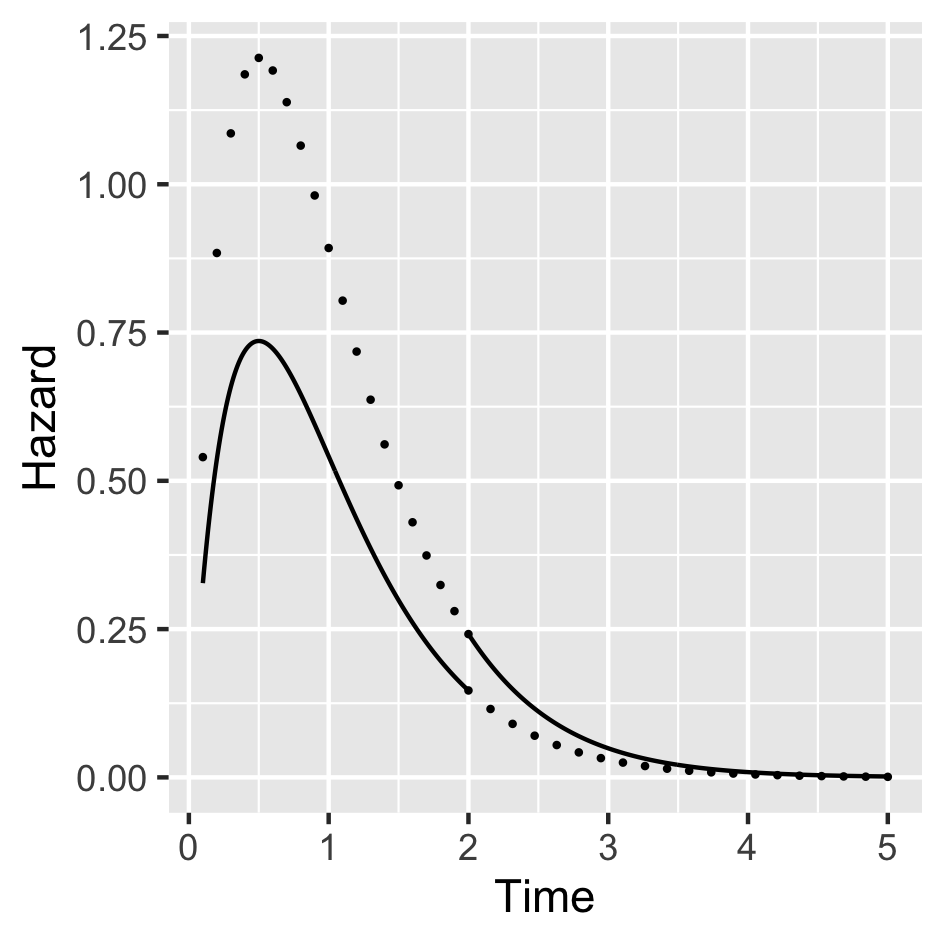
\includegraphics[width=7.5cm]{fig/tdcox.png}
	}
	\end{frame}

	\begin{frame}
	\frametitle{Parametric Models: Parametric Hazard Function}
	\begin{itemize}
	\item Parametric baseline hazard function, i.e, $h_0(t; \lambda)$
	\item Hazard function can be estimated more efficiently than semiparametric models
	\item Hazard function:
	\begin{eqnarray*}
	h(t,X_i) = h_0(t; \lambda) \exp(X_i \beta)
	\end{eqnarray*}
	\item Likelihood:
	\begin{eqnarray*}
	\prod_{i:\delta_i = 1} f(T_i; \beta, \lambda) \prod_{i:\delta_i = 0} S(C_i; \beta, \lambda)
	\end{eqnarray*}

	\end{itemize}

	\end{frame}

	\begin{frame}
	\frametitle{Parametric Hazard Function}
	\centering{
	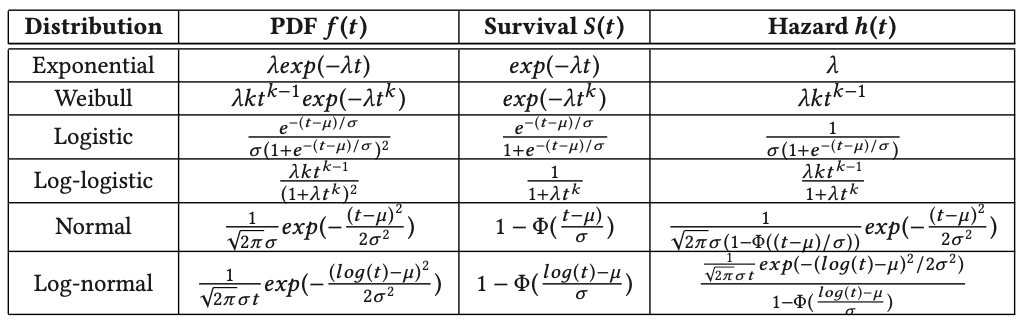
\includegraphics[width=\textwidth]{fig/Wang_et_al_Tab4.png}
	}
	\end{frame}
	
	\begin{frame}
	\frametitle{Exponential distribution}
	\centering{
	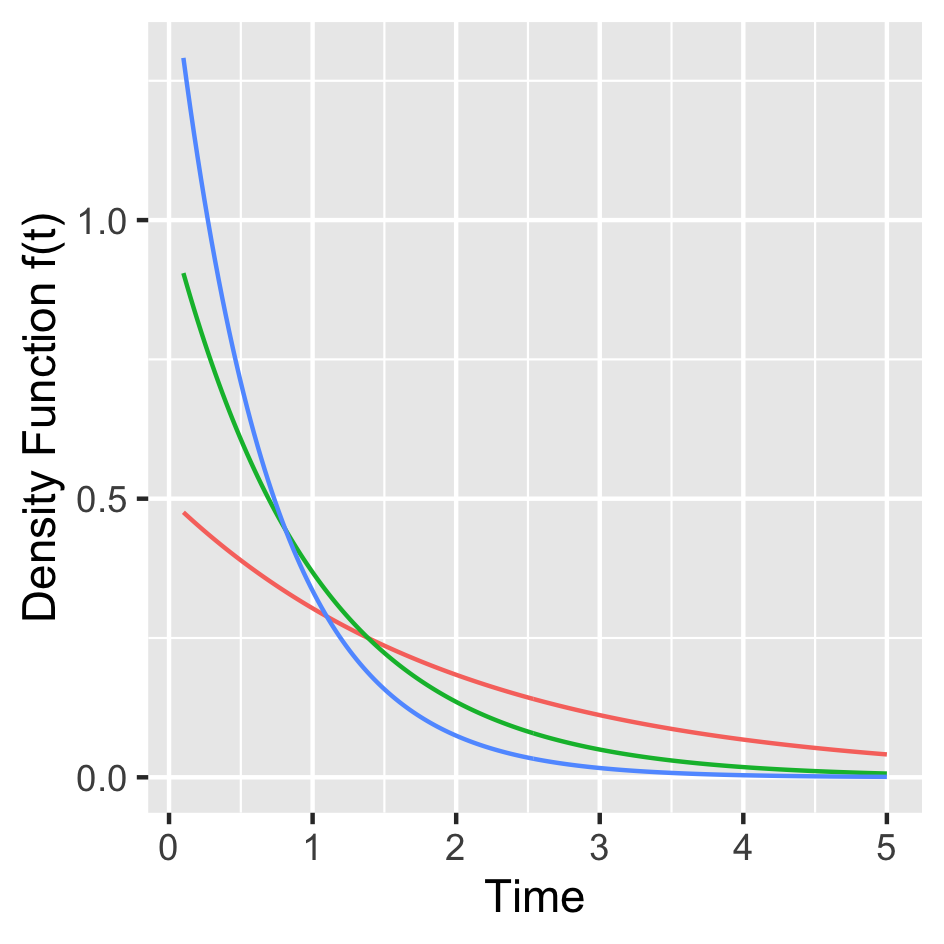
\includegraphics[width=7.5cm]{fig/exp.png}
	}
	\end{frame}

	\begin{frame}
	\frametitle{Parametric Models: Accelerated Failure Time Model}
	\begin{itemize}
	\item Event time is directly parameterized:
	\begin{eqnarray*}
	\log(T_i) = X_i \beta + \sigma \epsilon
	\end{eqnarray*}
	\item Likelihood:
	\begin{eqnarray*}
	\prod_{i:\delta_i = 1} f(T_i; \beta, \sigma) \prod_{i:\delta_i = 0} S(C_i; \beta, \sigma)
	\end{eqnarray*}

	\end{itemize}

	\end{frame}

	\begin{frame}
	\frametitle{Machine Learning Methods}
	\begin{itemize}
	\item Available methods:
	\begin{itemize}
	\item Regularized Cox models
	\item Survival trees
	\item Bayesian methods
	\item Neural networks
	\item Support vector machines

	\end{itemize}
	\item Machine learning methods primarily aim to build prediction models
	\item Causal inference framework is still in its infancy

	\end{itemize}

	\end{frame}

	\begin{frame}
	\frametitle{Survival Trees}
	\centering{
	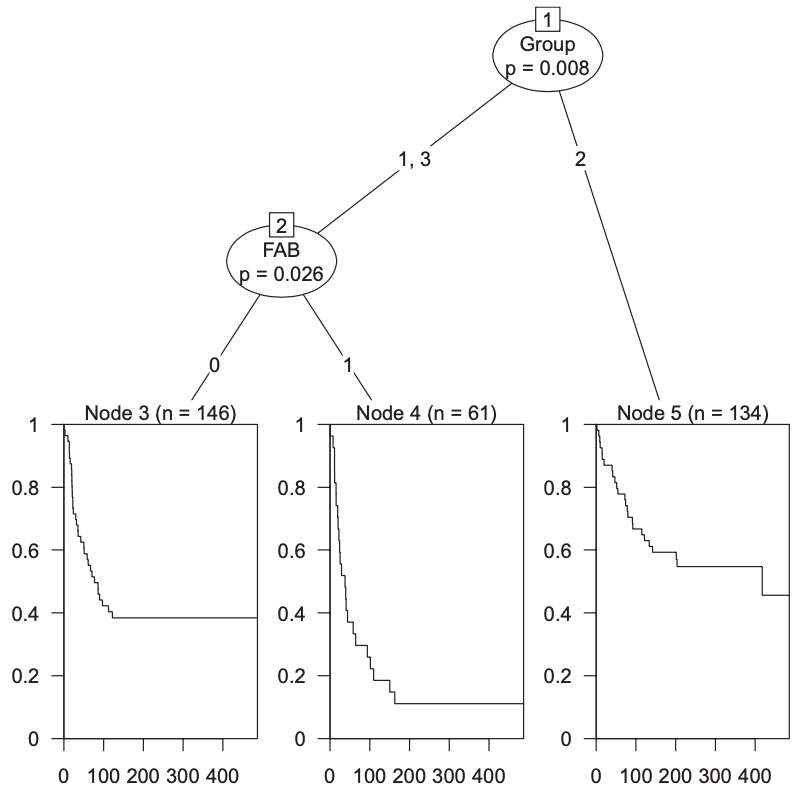
\includegraphics[width=7.5cm]{fig/Fu_et_al_Fig3_L.png}
	}
	\end{frame}

	\section{Related Topics}

	\begin{frame}
	\frametitle{Performance Measures: C-index}
	\begin{itemize}
	\item Compare the rankings of observed and predicted survival times
	\item Concordance probability:
	\begin{eqnarray*}
	c = \Pr(\hat{y_i} > \hat{y_j} | y_i > y_j)
	\end{eqnarray*}
	\item Estimator of C-index for Cox models:
	\begin{eqnarray*}
	\hat{c} = \frac{1}{num} \sum_{i:\delta_i = 1} \sum_{j:y_i < y_j} I(X_i \hat{\beta} > X_j \hat{\beta})
	\end{eqnarray*}
	$num$: number of all comparable pairs
	\item If $y_i$ is binary, C-index $=$ AUC

	\end{itemize}

	\end{frame}

	\begin{frame}
	\frametitle{C-index}
	\centering{
	$y_1 < y_2 < y_3 < y_4 < y_5$\\
	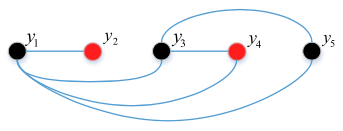
\includegraphics[width=8cm]{fig/Wang_et_al_Fig4b.png}\\
	Black: event observed\\
	Red: censored\\
	Edges: possible ranking comparisons
	}
	\end{frame}

	\begin{frame}
	\frametitle{Performance Measures: Brier Score}
	\begin{itemize}
	\item Compare the observed and predicted event occurrence before time $t$
	\item $z_i(t)$: indicator of event before $t$
	\item $\hat{z}_i(t)$: predicted probability of event before $t$
	\item Brier score at $t$:
	\begin{eqnarray*}
	BS(t) = \frac{1}{N} \sum_{i=1}^N \{\hat{z}_i(t) - z_i(t) \}
	\end{eqnarray*}
	\item Censored information can be incorporated

	\end{itemize}

	\end{frame}

	\begin{frame}
	\frametitle{Competing Risks}
	\begin{itemize}
	\item $D_i \in \{1 \dots K \}$: $i$'s cause of event
	\item Cause-specific density:
	\begin{eqnarray*}
	f_k(t) = \lim_{\Delta t \to 0}\frac{\Pr(t \leq T < t + \Delta t, D = k)}{\Delta t}
	\end{eqnarray*}
	\item Cumulative incidence function (CIF):
	\begin{eqnarray*}
	I_k(t) = \int_0^t f_k(\tau)d\tau = \Pr\{T \leq t, D = k \}
	\end{eqnarray*}
	\item Can we estimate the effect of $X$ on CIF?

	\end{itemize}

	\end{frame}

	\begin{frame}
	\frametitle{Competing Risks}
	\begin{itemize}
	\item Consider cause-specific hazard function:
	\begin{eqnarray*}
	h_k^{cs} (t) = \lim_{\Delta t \to 0}\frac{\Pr(t \leq T < t + \Delta t, D = k | T \geq t)}{\Delta t}
	\end{eqnarray*}
	\item $h_k^{cs} (t)$ can be estimated using the Cox model:
	\begin{eqnarray*}
	h_k^{cs} (t, X_i) = h_{k0}^{cs} (t) \exp(X_i \beta_k^{cs})
	\end{eqnarray*}
	\item Effect of $X$ on CIF cannot be inferred from $\beta_k^{cs}$

	\end{itemize}

	\end{frame}

	\begin{frame}
	\frametitle{Competing Risks}
	\begin{itemize}
	\item Alternative is subdistribution hazard function\footnote{Fine and Gray (1999, JASA)}:
	\begin{eqnarray*}
	h_k^{sd} (t) = \lim_{\Delta t \to 0}\frac{\Pr(t \leq T < t + \Delta t, D = k | A)}{\Delta t},
	\end{eqnarray*}
	where $A = \{T \geq t \text{ or } (T < t, D \neq k)\}$
	\item $h_k^{sd} (t)$ can be estimated using the Cox model:
	\begin{eqnarray*}
	h_k^{sd} (t, X_i) = h_{k0}^{sd} (t) \exp(X_i \beta_k^{sd})
	\end{eqnarray*}

	\end{itemize}

	\end{frame}

	\begin{frame}
	\frametitle{Competing Risks}
	\begin{itemize}
	\item Effect of $X$ on CIF can be inferred from $\beta_k^{sd}$ as
	\begin{eqnarray*}
	&\phantom{=}& \log(-\log(1 - I_k(t,X)))\\
	&=& \log(-\log(1 - I_{k0}(t))) + X \beta_k^{sd}
	\end{eqnarray*}
	\item When the probability of an event is low, then the logistic link function and the complementary log‐log link function are very similar.
	\item Thus, if this is the case, $\beta_k^{sd}$ can be interpreted as odds ratios for the CIF.

	\end{itemize}

	\end{frame}

	\begin{frame}
	\frametitle{Competing Risks with Time-Dependent Covariates\footnote{Geskus (2011, Biometrics)}}
	\begin{itemize}
	\item Individuals with time-dependent covariates can be incorporated in a competing risk model.
	\item Split their observation periods into periods where the covariates do not vary with time.
	\item Consider left truncation as well as right censoring in the estimation.

	\end{itemize}

	\end{frame}

	\begin{frame}
	\frametitle{Competing Risks with Time-Dependent Covariates}
	\begin{itemize}
	\item ``Weights'' of individuals who experienced competing events need to be adjusted for left truncation and right censoring.
	\item Each $i$ has weight $w_i(T_j)$ at $T_j$ given by:
	\begin{eqnarray*}
	w_i(T_j) =
	\begin{cases}
	1 & \text{if ``at risk'' at $T_j$}\\
	\frac{\Pr(C \geq T_j) \Pr(L < T_j)}{\Pr(C \geq T_j') \Pr(L < T_j')} & \text{if $B$}\\
	0 & \text{otherwise},
	\end{cases}
	\end{eqnarray*}
	where $L$ is left entry time and $B = \{i \text{ had competing events at } T_j' < T_j\}$.

	\end{itemize}

	\end{frame}

	\begin{frame}
	\frametitle{Competing Risks with Time-Dependent Covariates: Estimation Procedure}
	\begin{itemize}
	\item Split each observation period into periods where the covariates do not vary with time.
	\begin{itemize}
	\item Some rows will have left entry time $> 0$.
	\end{itemize}
	\item Attach weights to the observations.
	\begin{itemize}
	\item Individuals who experienced competing events will have many time-varying weights.
	\end{itemize}
	\item Apply survival analysis program that can handle left truncation in addition to right censoring.

	\end{itemize}

	\end{frame}

	\begin{frame}
	\frametitle{Multi-State Models: Continuous-Time Markov Model\footnote{Kalbfleisch and Lawless (1985, JASA)}}
	\begin{itemize}
	\item Survival analysis models usually deal with transition from one state to another.
	\item In some cases, modeling transitions between multiple states may be valuable.
	\item Continuous-time Markov model can be used for this purpose.
	\end{itemize}
	\end{frame}

	\begin{frame}
	\frametitle{Continuous-Time Markov Model}
	\begin{itemize}
	\item Continuous-time Markov model can be viewed as an extension of a parametric Cox model.
	\item $S_i(t) \in \{1 \dots R \}$: $i$'s state at time $t$

	\end{itemize}
	\end{frame}

	\begin{frame}
	\frametitle{Continuous-Time Markov Model}
	\begin{itemize}
	\item Hazard (instantaneous risk) of moving from state $r$ to state $r'$ is assumued to be:
	\begin{eqnarray*}
	h_{rr'}(t) = \lim_{\Delta t \to 0} \frac{\Pr(S(t + \Delta t) = r | S(t) = r')}{\Delta t}
	\end{eqnarray*}
	\item $h_{rr'}(t)$ is estimated using the same parameterization as the parametric Cox model:
	\begin{eqnarray*}
	h_{rr'} (t, X_i(t)) = h_{rr'0}(t; \lambda_{rr'}) \exp(X_i(t) \beta_{rr'})
	\end{eqnarray*}

	\end{itemize}
	\end{frame}

	\begin{frame}
	\frametitle{Continuous-Time Markov Model}
	\centering{
	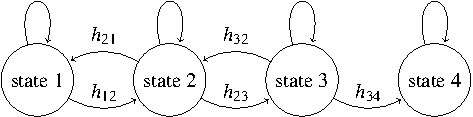
\includegraphics[width=\textwidth]{fig/markov/markov-crop.pdf}
	}
	\end{frame}

	\section{Applications}

	\begin{frame}
	\frametitle{Kaito et al. (2020, Blood Adv.)}
	\centering{
	
\includegraphics[width=\textwidth]{fig/Kaito_et_al_title.png}
	}
	\end{frame}

	\begin{frame}
	\frametitle{Introduction}
	\begin{itemize}
	\item Investigated the heterogeneous impact of CMV reactivation on NRM in hematopoietic stem cell transplantation.
	\item Used time-dependent Cox model considering competing risks.
	\item Heterogeneous impact was quantified by interaction terms.

	\end{itemize}
	\end{frame}

	\begin{frame}
	\frametitle{Heterogeneous Treatment Effect}
	\begin{itemize}
	\item Treatment effects may vary across the levels of baseline characteristics.
	\item Subgroup analysis is one way to investigate heterogeneous treatment effects (HTEs).
	\item However, subgroups can be very small if there are a lot of baseline characteristics.
	\item Statistical tests of interactions between the treatment and baseline characteristics can be a solution.

	\end{itemize}
	\end{frame}

	\begin{frame}
	\frametitle{Heterogeneous Treatment Effect}
	\begin{itemize}
	\item $D$: treatment
	\item $X$: baseline characteristics
	\item Statistical tests of interactions:
	\begin{eqnarray*}
	y = X \beta + D * X \gamma
	\end{eqnarray*}
	\item Significant $\gamma$ indicates the HTE.
	\item In this study,
	\begin{eqnarray*}
	\text{NRM} = X \beta + \text{CMV} * X \gamma.
	\end{eqnarray*}

	\end{itemize}
	\end{frame}

	\begin{frame}
	\frametitle{Heterogeneous Treatment Effect}
	\centering{
	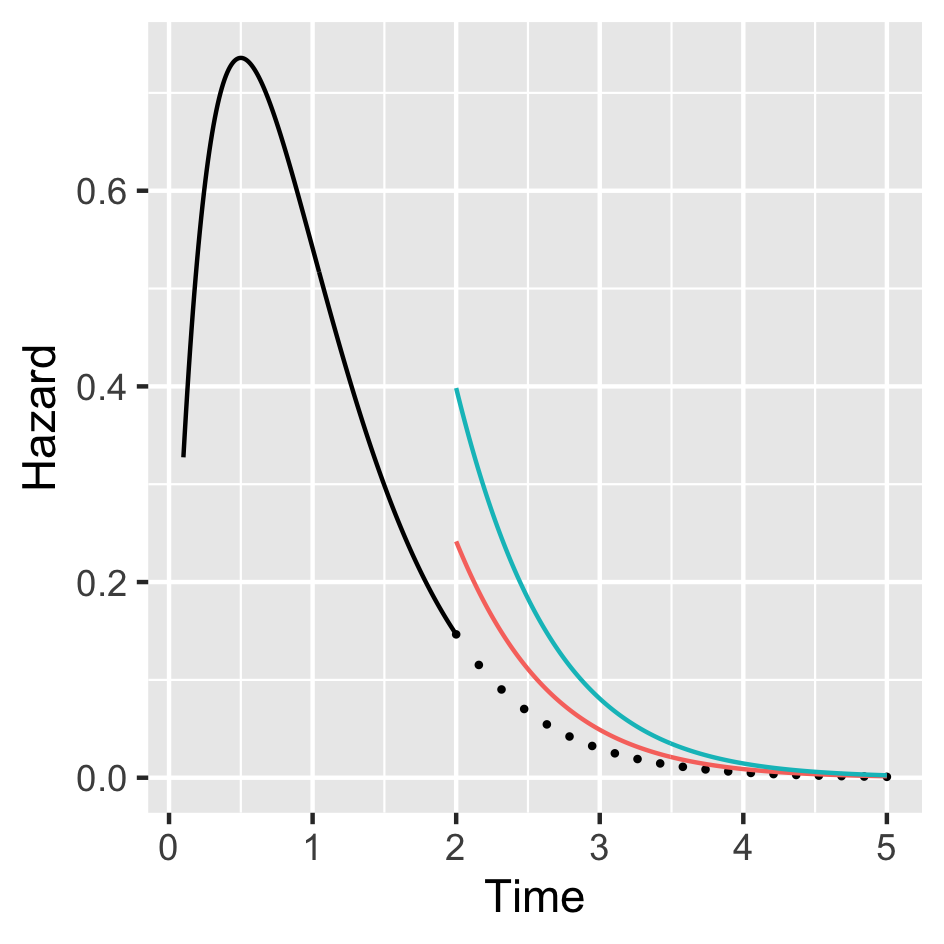
\includegraphics[width=7.5cm]{fig/htecox.png}
	}
	\end{frame}

	\begin{frame}
	\frametitle{Scoring model for CMV reactivation}
	\begin{itemize}
	\item Cumulative incidence of CMV reactivation was evaluated considering relapse and NRM as competing risks.
	\item Scoring model for CMV reactivation was developed and assessed by landmark analysis at day 100.

	\end{itemize}
	\end{frame}

	\begin{frame}
	\frametitle{Scoring model for CMV reactivation}
	Significant factors (HR $>$ 1):
	\begin{itemize}
	\item Recipient positive/donor negative CMV serology
	\item Recipient positive/donor positive CMV serology
	\item TCD {\it in vivo}
	\item HLA disparity
	\item $\geq$ 50 years
	\item Transplant from an unrelated donor
	\item TBI
	\item Older transplant year

	\end{itemize}
	\end{frame}

	\begin{frame}
	\frametitle{Scoring model for CMV reactivation}
	Significant factors (HR $<$ 1):
	\begin{itemize}
	\item Tacrolimus-based GVHD prophylaxis regimen
	\item CB

	\end{itemize}
	\end{frame}

	\begin{frame}
	\frametitle{Scoring model for CMV reactivation}
	\centering{
	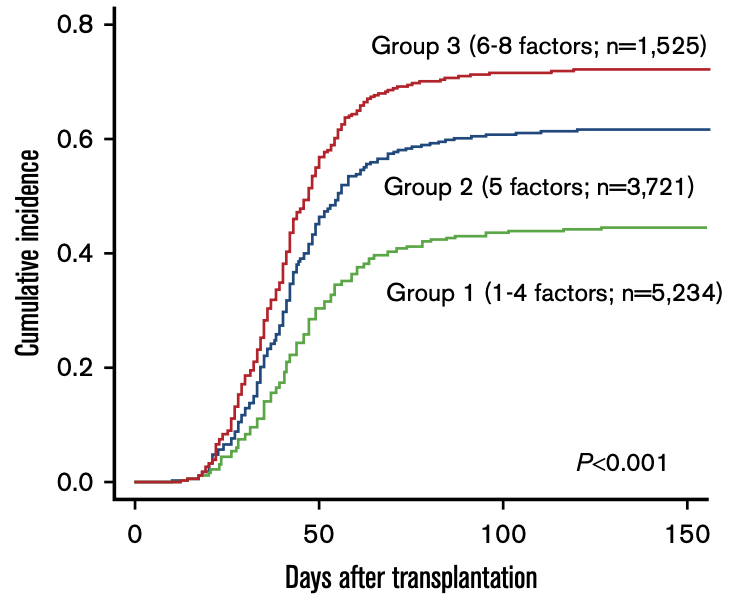
\includegraphics[height=7.5cm]{fig/Kaito_et_al_Fig1B.png}
	}
	\end{frame}

	\begin{frame}
	\frametitle{Impact of CMV reactivation on NRM}
	\centering{
	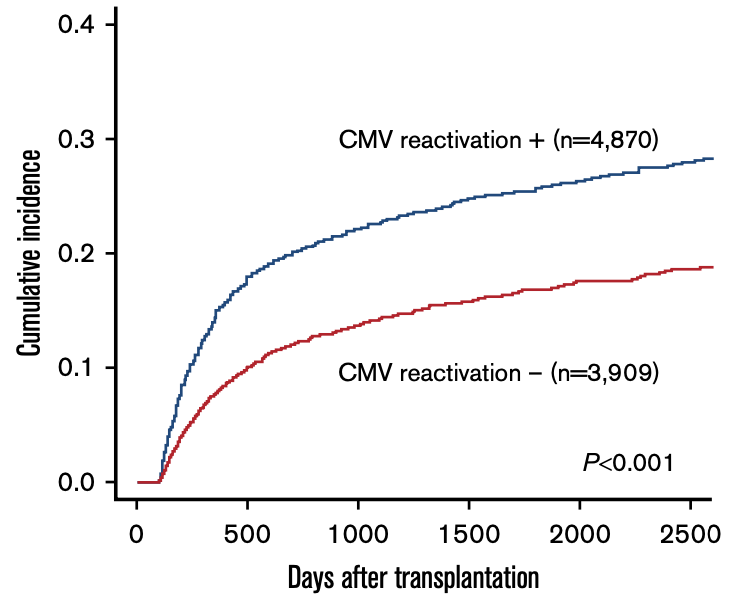
\includegraphics[height=7.5cm]{fig/Kaito_et_al_Fig1A.png}
	}
	\end{frame}

	\begin{frame}
	\frametitle{Impact of CMV reactivation on NRM}
	\centering{
	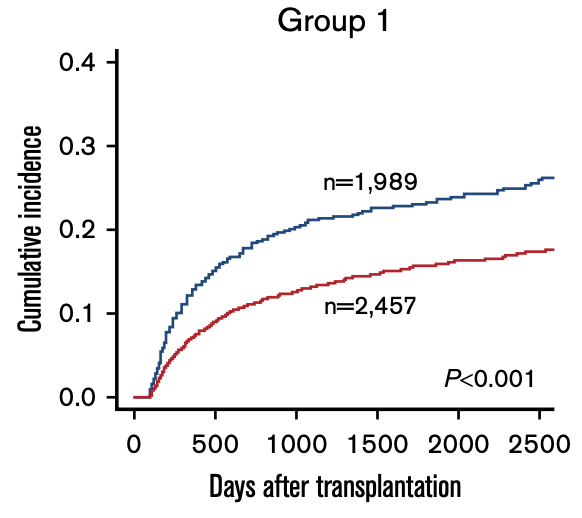
\includegraphics[height=7.5cm]{fig/Kaito_et_al_Fig2A.png}
	}
	\end{frame}

	\begin{frame}
	\frametitle{Impact of CMV reactivation on NRM}
	\centering{
	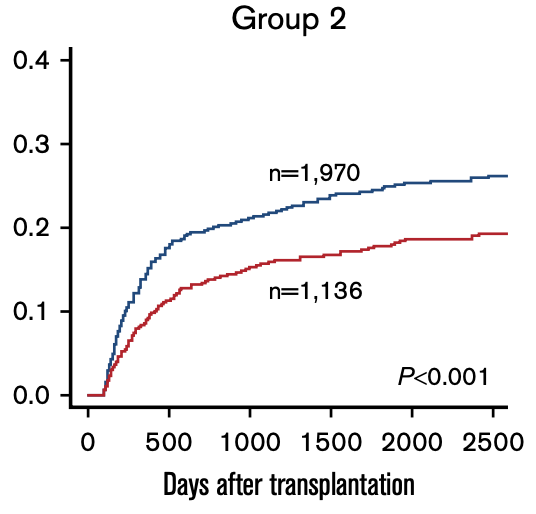
\includegraphics[height=7.5cm]{fig/Kaito_et_al_Fig2B.png}
	}
	\end{frame}

	\begin{frame}
	\frametitle{Impact of CMV reactivation on NRM}
	\centering{
	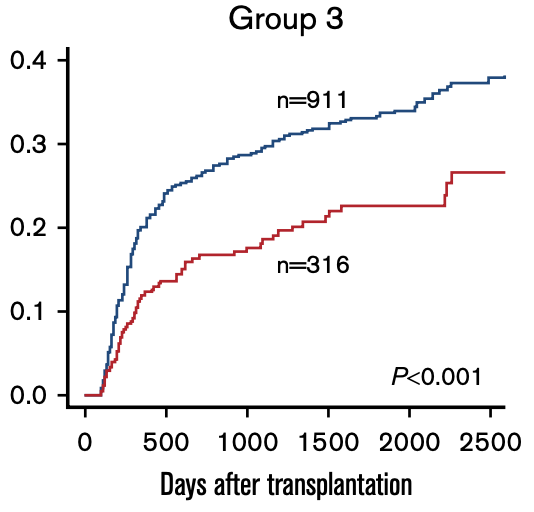
\includegraphics[height=7.5cm]{fig/Kaito_et_al_Fig2C.png}
	}
	\end{frame}

	\begin{frame}
	\frametitle{Heterogeneous impact}
	\begin{itemize}
	\item Cumulative incidence of NRM was evaluated considering relapse as a competing risk and CMV reactivation as a time-dependent covariate.
	\item Interaction terms between CMV reactivation and baseline characteristics were included in the model.
	\item Scoring model for the heterogeneous impact of CMV reactivation on NRM was developed and assessed by landmark analysis at day 100.

	\end{itemize}
	\end{frame}

	\begin{frame}
	\frametitle{Heterogeneous impact}
	Significant factors (HR $>$ 1):
	\begin{itemize}
	\item CML

	\end{itemize}
	Significant factors (HR $<$ 1):
	\begin{itemize}
	\item Poor PS
	\item Transplantation from HLA-mismatched donors
	\item High disease risk

	\end{itemize}

	\end{frame}

	\begin{frame}
	\frametitle{Heterogeneous impact}
	\centering{
	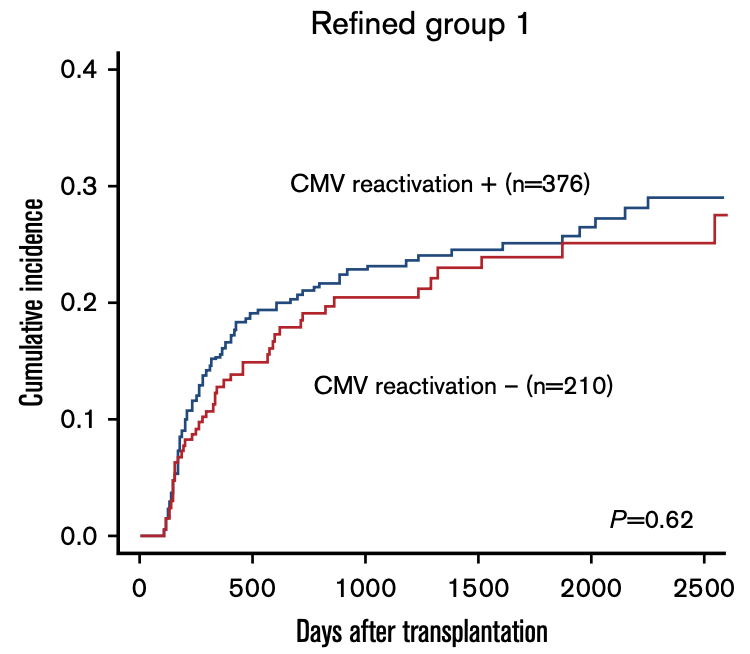
\includegraphics[height=7.5cm]{fig/Kaito_et_al_Fig3A.png}
	}
	\end{frame}

	\begin{frame}
	\frametitle{Heterogeneous impact}
	\centering{
	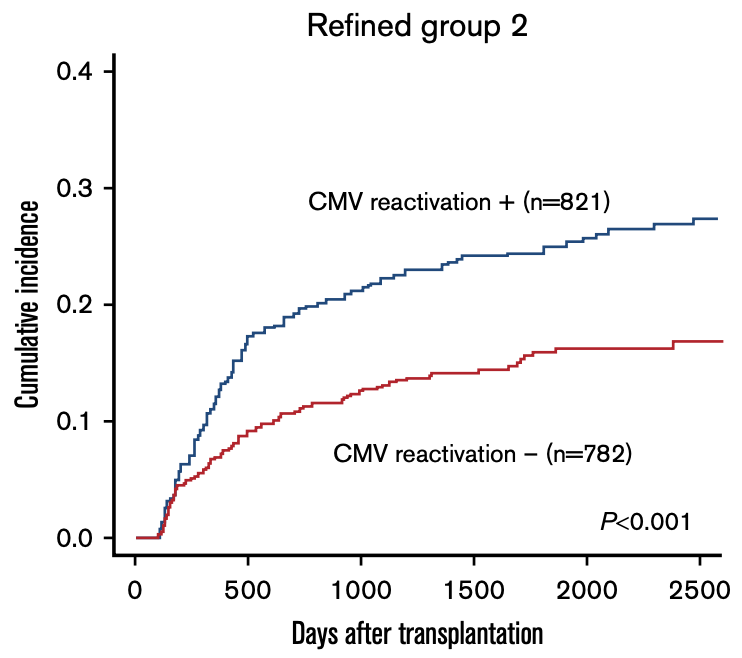
\includegraphics[height=7.5cm]{fig/Kaito_et_al_Fig3B.png}
	}
	\end{frame}

	\begin{frame}
	\frametitle{Taguchi et al. (2020, Cancers)}
	\centering{
	
\includegraphics[width=\textwidth]{fig/Taguchi_et_al_title.png}
	}
	\end{frame}

	\begin{frame}
	\frametitle{Introduction}
	\begin{itemize}
	\item Investigated the prognosis of hrHPV-related cervical lesions.
	\item CIN has a natural history of bidirectional transition between different states.
	\item Cox models assuming a unidirectional disease progression may oversimplify CIN fate.
	\item Application of continuous-time Markov model to this situation may be of interest.

	\end{itemize}
	\end{frame}

	\begin{frame}
	\frametitle{Samples}
	\centering{
	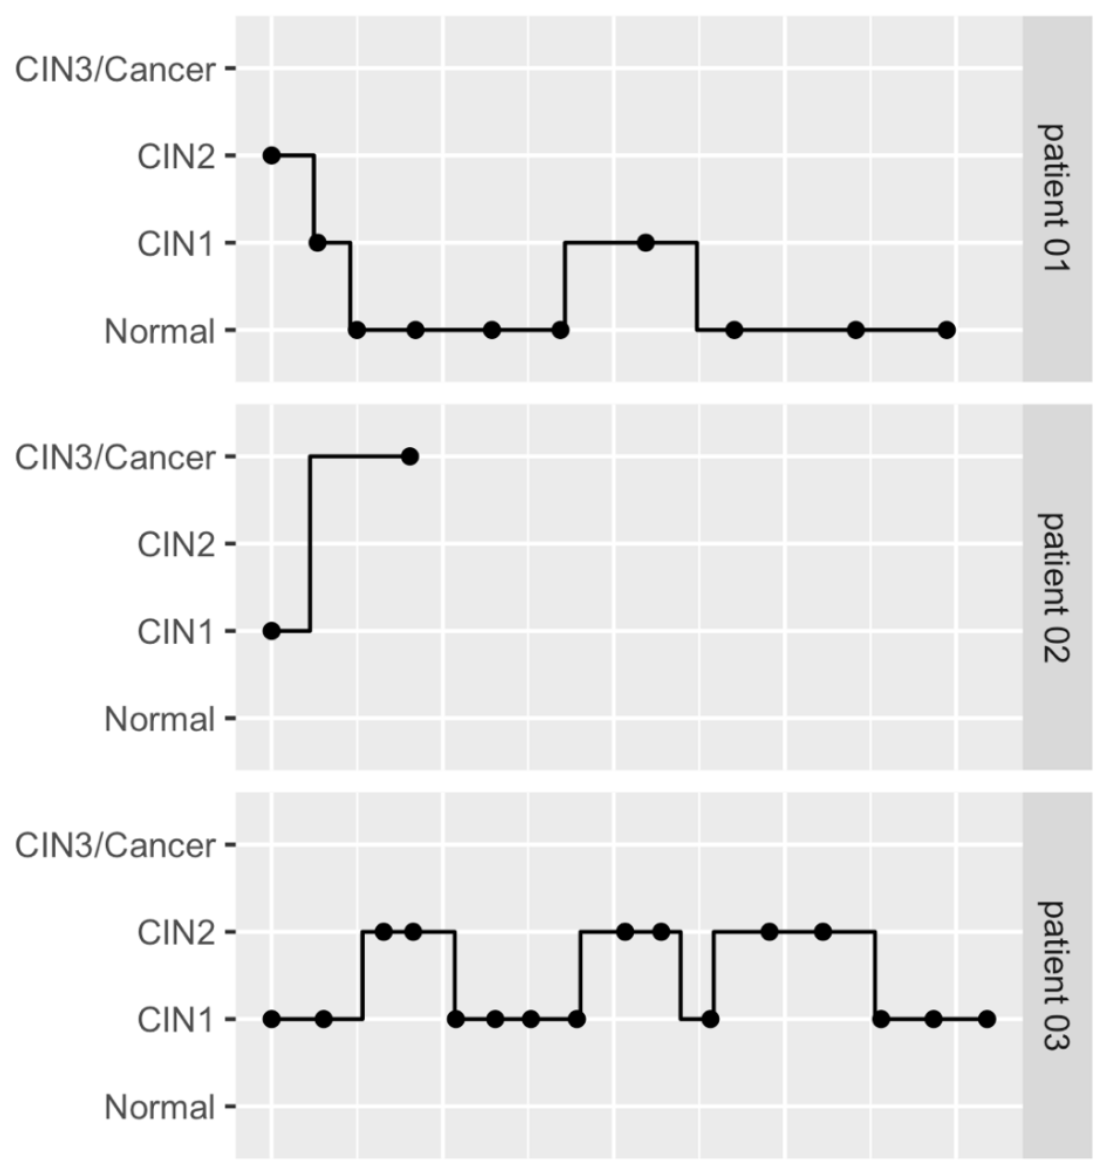
\includegraphics[height=7.5cm]{fig/Taguchi_et_al_Fig3.png}
	}
	\end{frame}

	\begin{frame}
	\frametitle{Summary of transitions}
	\centering{
	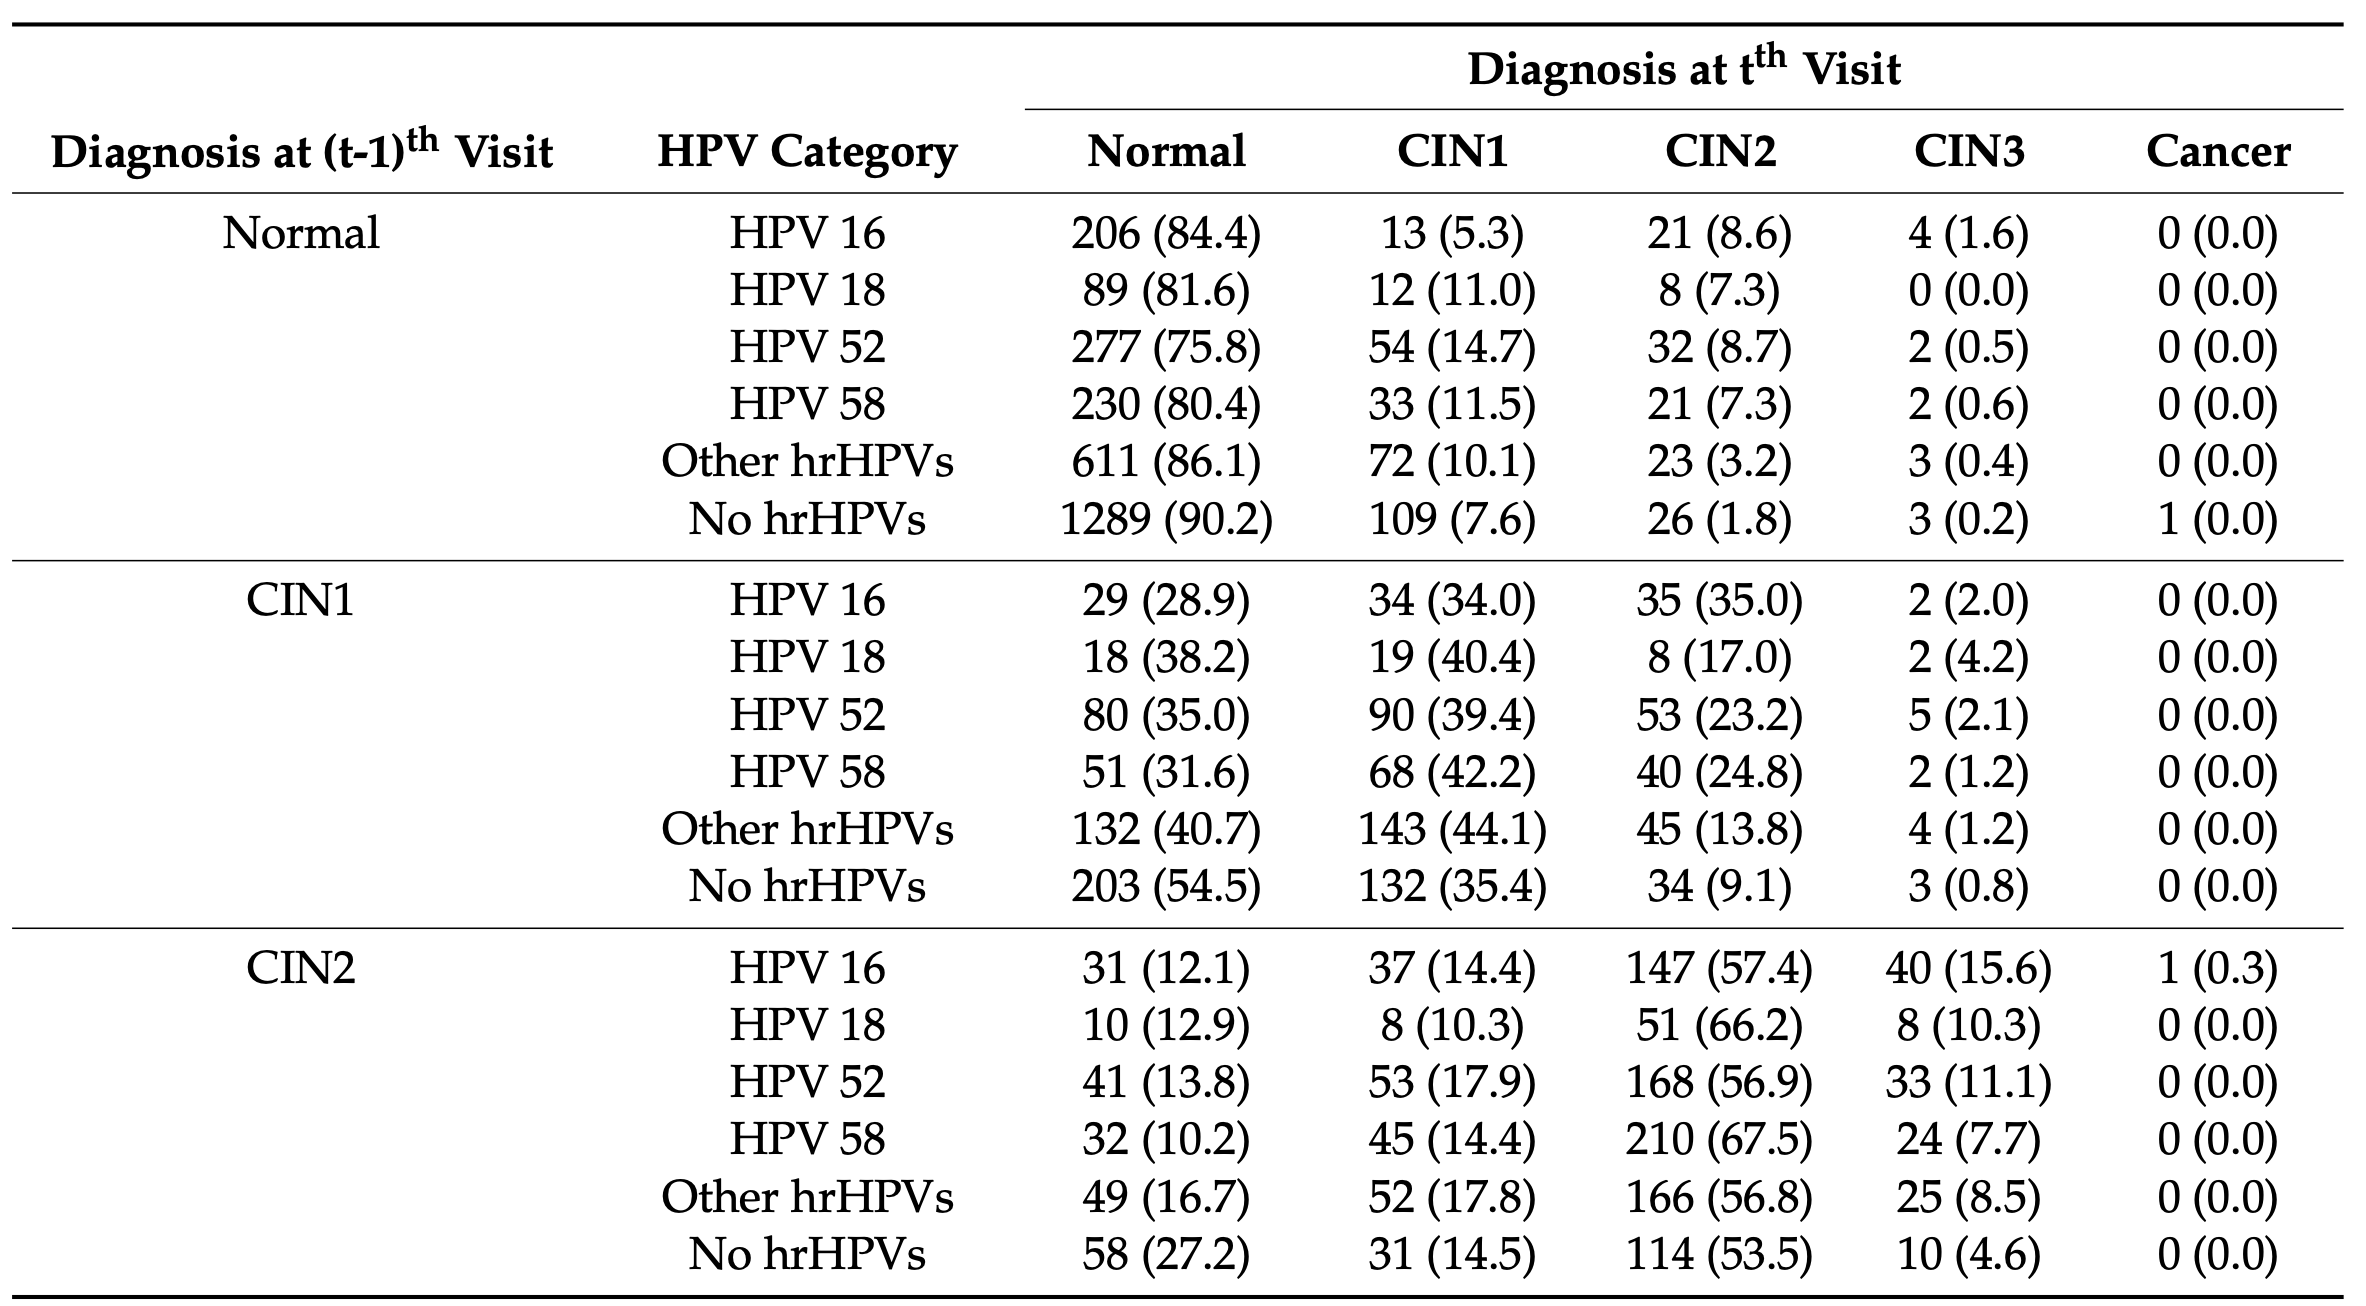
\includegraphics[width=14cm]{fig/Taguchi_et_al_Tab2.png}
	}
	\end{frame}

	\begin{frame}
	\frametitle{Continuous-time Markov model}
	\centering{
	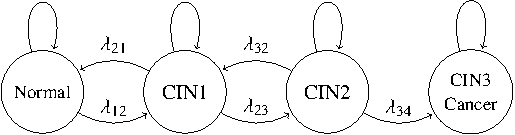
\includegraphics[width=\textwidth]{fig/Taguchi_et_al_Fig2.pdf}
	}
	\end{frame}

	\begin{frame}
	\frametitle{Continuous-Time Markov Model}
	\begin{itemize}
	\item Parameterization of the hazard function:
	\begin{eqnarray*}
	\lambda_{rr'} (t, \text{HPV}) = \lambda_{rr'0}^{\text{HPV}}
	\end{eqnarray*}
	\item Hazards were assumed to be constant across time.
	\item Hazards were estimated for each HPV category.
	\item It was challenging to find a parameterization where the estimation converges.

	\end{itemize}
	\end{frame}

	\begin{frame}
	\frametitle{Predicted 2-year transition probabilities}
	\centering{
	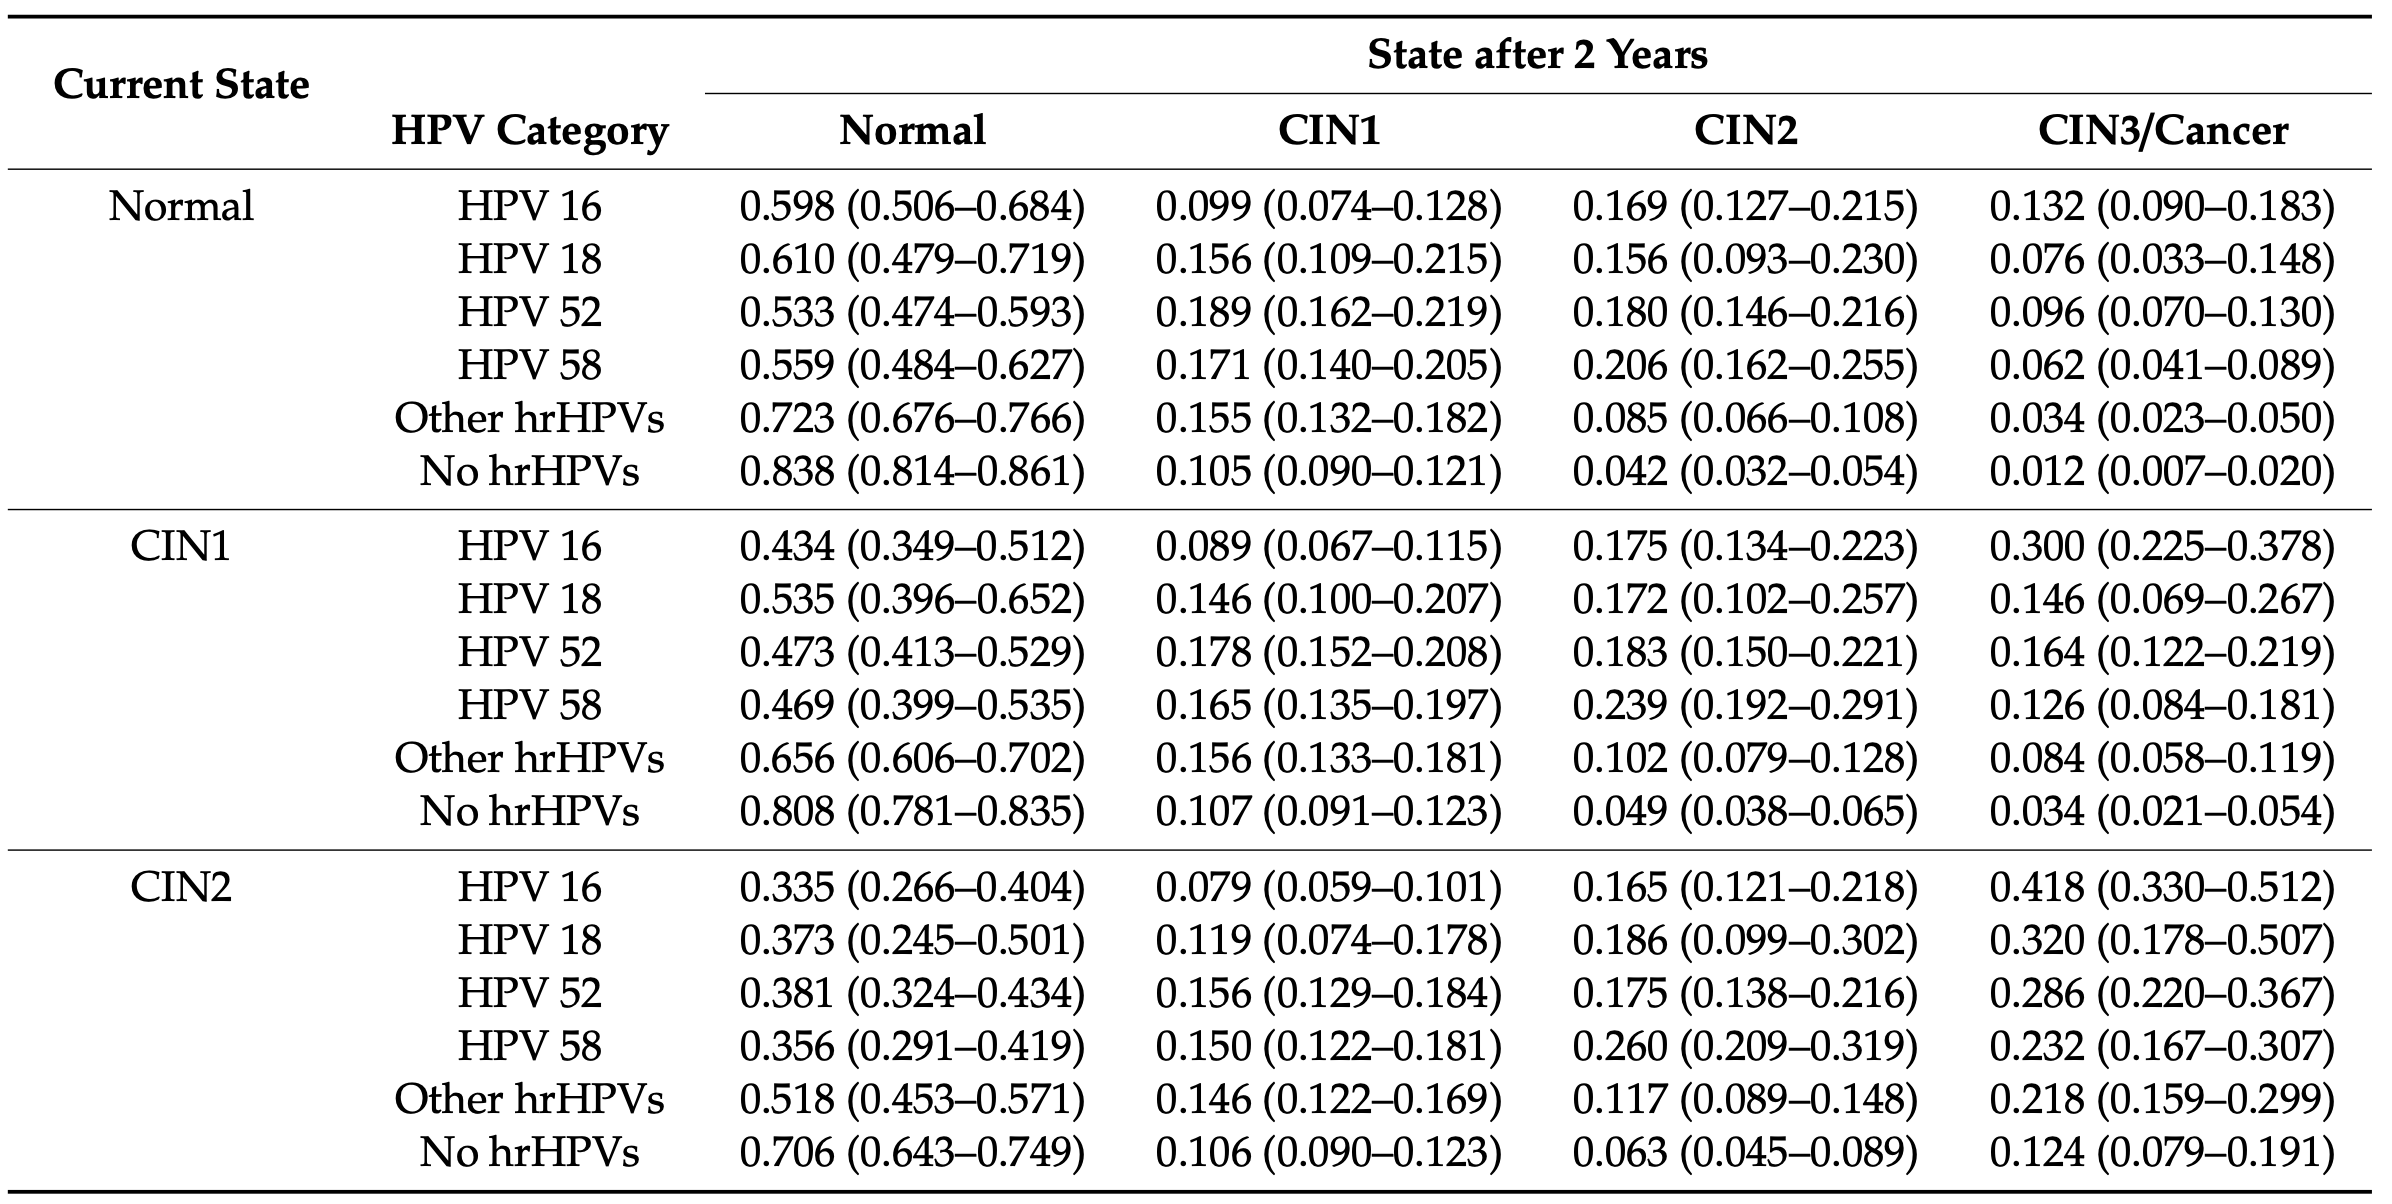
\includegraphics[width=15cm]{fig/Taguchi_et_al_Tab3.png}
	}
	\end{frame}

	\begin{frame}
	\frametitle{Observed and simulated prevalence}
	\centering{
	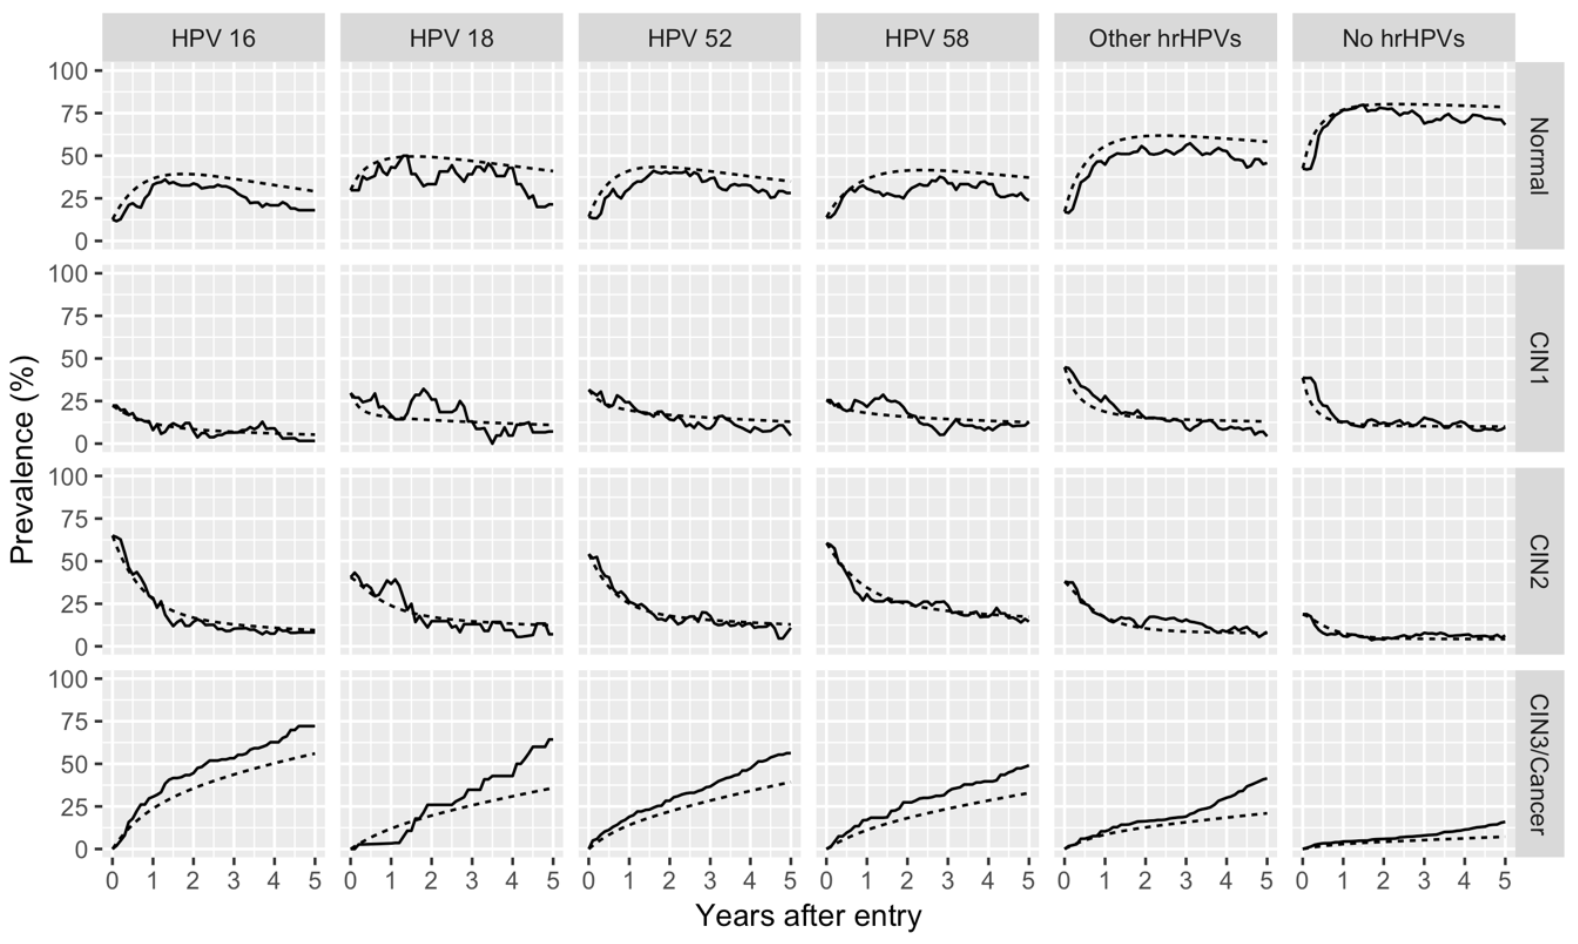
\includegraphics[width=13cm]{fig/Taguchi_et_al_Fig1.png}
	}
	\end{frame}



















\end{document}
